<<<<<<< HEAD
\section{Discuss�o sobre a melhor topologia para corre��o de fator de pot�ncia}

\begin{figure}[!htbp]
	\centering
	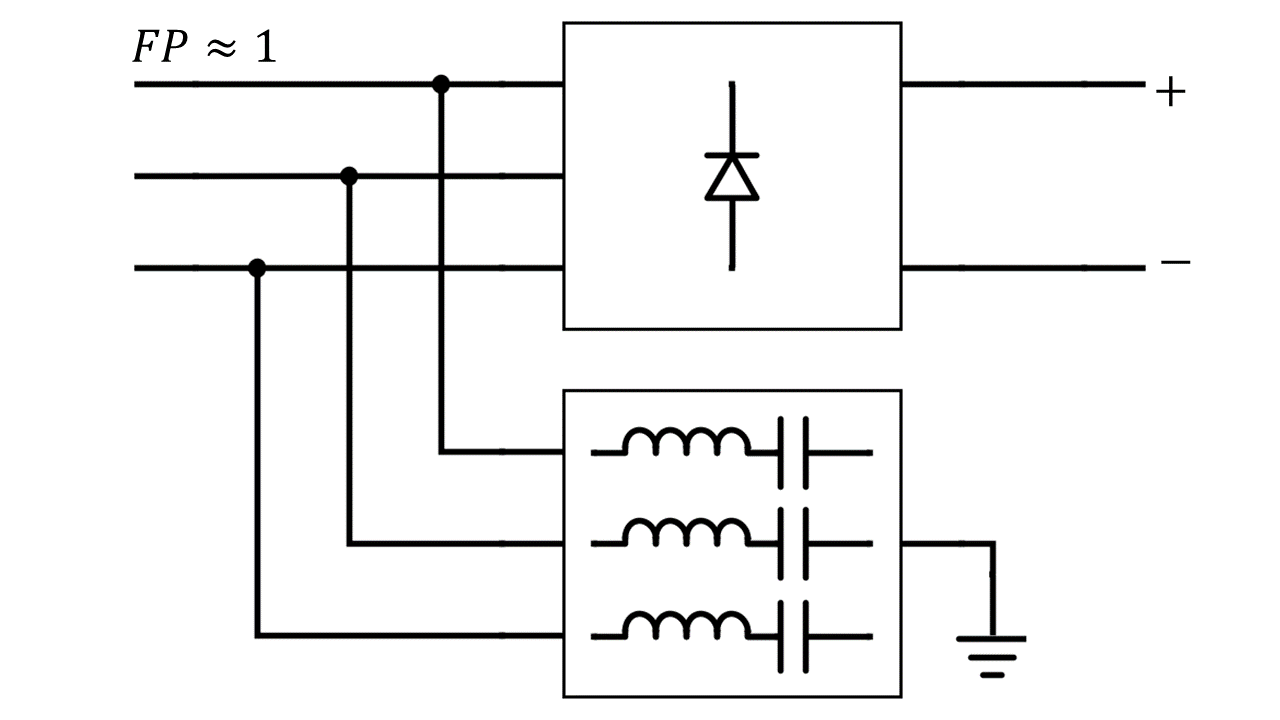
\includegraphics[width=0.75\textwidth]{Cap2/Figuras/sch_filtro_passivo.png}
	\caption{Filtro Passivo}
	\label{fig:sch_filtro_passivo}
\end{figure}

\begin{figure}[!htbp]
	\centering
	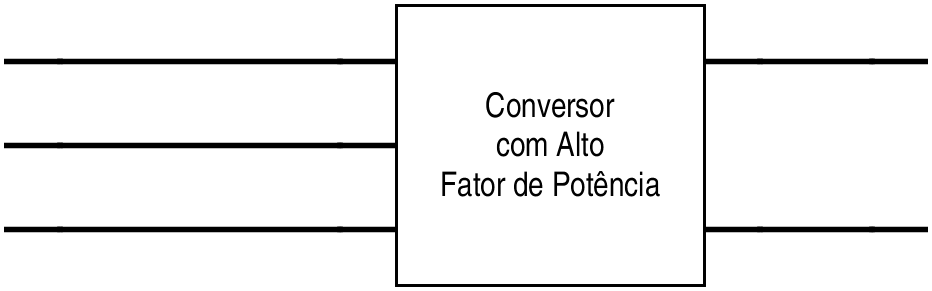
\includegraphics[width=0.75\textwidth]{Cap2/Figuras/sch_PFC.png}
	\caption{Filtro PFC}
	\label{fig:sch_PFC}
\end{figure}

\begin{figure}[!htbp]
	\centering
	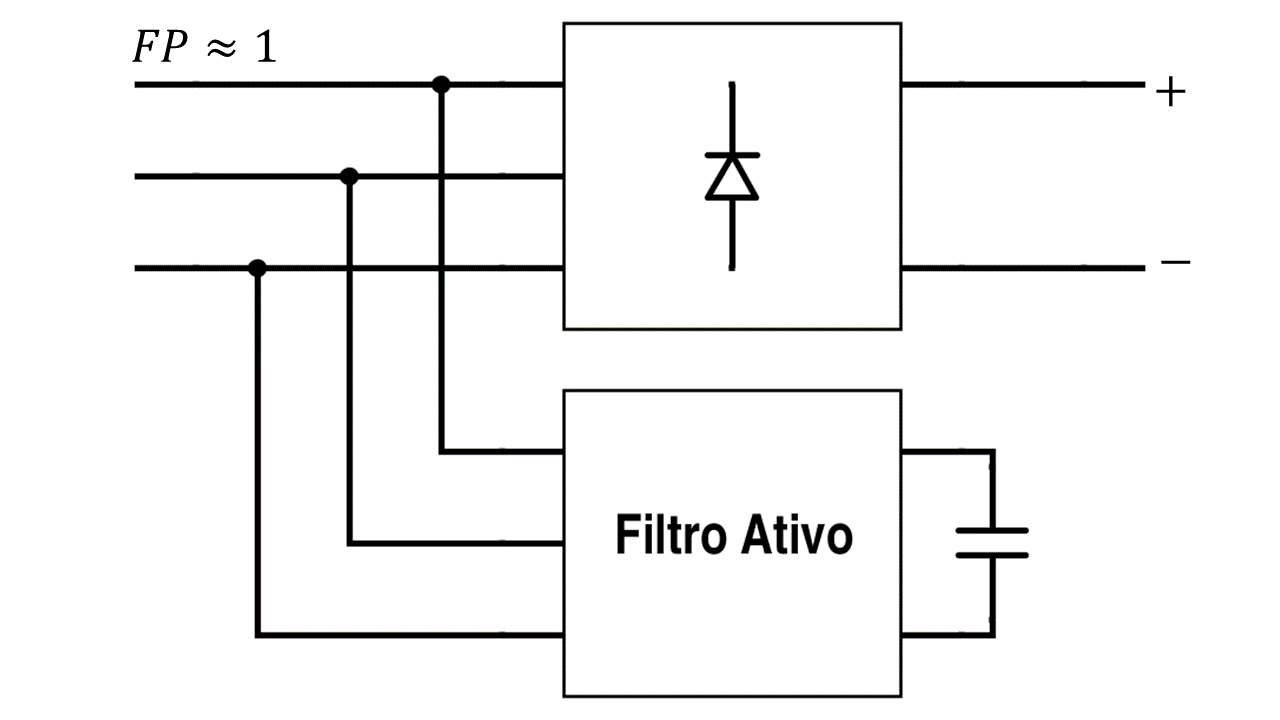
\includegraphics[width=0.75\textwidth]{Cap2/Figuras/sch_filtro_ativo.png}
	\caption{Filtro Ativo}
	\label{fig:sch_filtro_ativo}
\end{figure}

=======
\section{Discuss�o sobre a melhor topologia para corre��o de fator de pot�ncia}

Para a opera��o segura e de acordo com o cumprimento dos requisitos aeron�uticos, s�o necess�rios procedimentos para suprimir o alto \textit{THD} nos sistema el�trico de uma aeronave, de modo que seus efeitos n�o sejam prejudiciais aos equipamentos instalados na rede. 
Dentre os diversos m�todos de mitiga��o de harm�nicas nas redes do sistema el�trico de uma aeronave, destacam-se diversas topologias onde cada uma possui suas vantagens, desvantagens e peculiaridades. Nesse trabalho ser� descrito duas classes de sistemas de controle de harm�nicas: os passivos e os ativos.

\subsection{Sistemas Passivos} 

A caracteriza��o de um sistema passivo d�-se pela aus�ncia de um controle ativo para o controle de comuta��o de dispositivos semicondutores. Neste tipo de sistema, na presen�a de semicondutores, a comuta��o � desempenhada por diodos, as quais n�o necessitam de comando de um controle externo para a que haja a abertura ou o bloqueio do fluxo de corrente entre seus terminais. Outro sistema passivo � dado por filtros casados com as harm�nicas de alta frequ�ncias do sistema. 

\begin{figure}[!htbp]
	\centering
	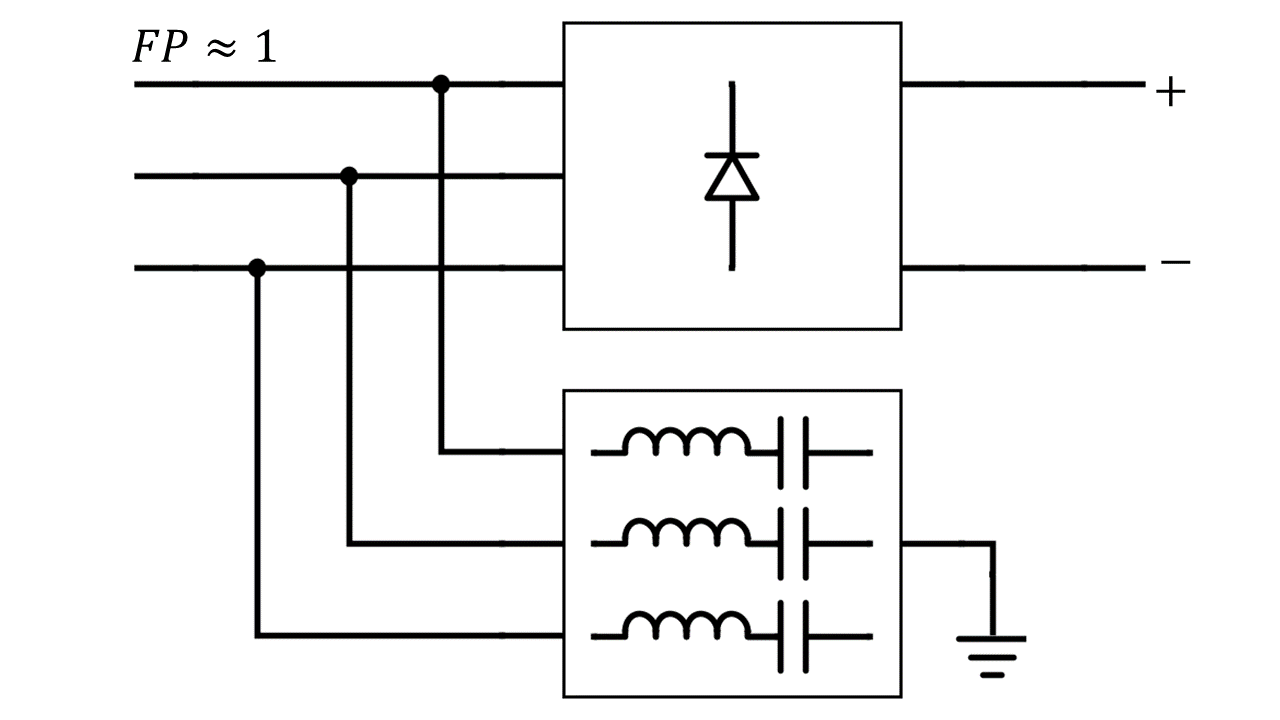
\includegraphics[width=0.65\textwidth]{Cap2/Figuras/sch_filtro_passivo.png}
	\caption{Filtro Passivo}
	\label{fig:sch_filtro_passivo}
\end{figure}

\begin{figure}[!htbp]
	\centering
	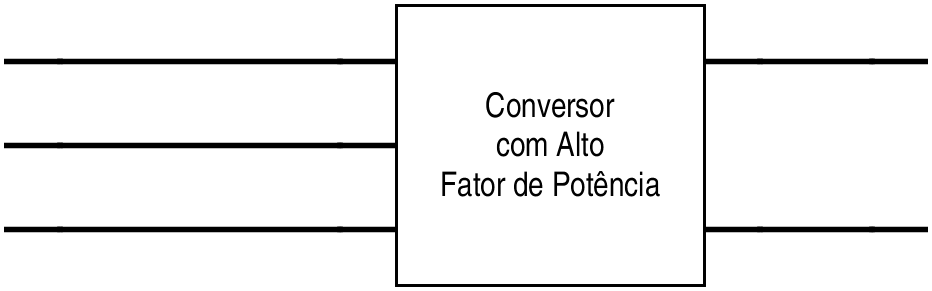
\includegraphics[width=0.65\textwidth]{Cap2/Figuras/sch_PFC.png}
	\caption{Filtro PFC}
	\label{fig:sch_PFC}
\end{figure}

\begin{figure}[!htbp]
	\centering
	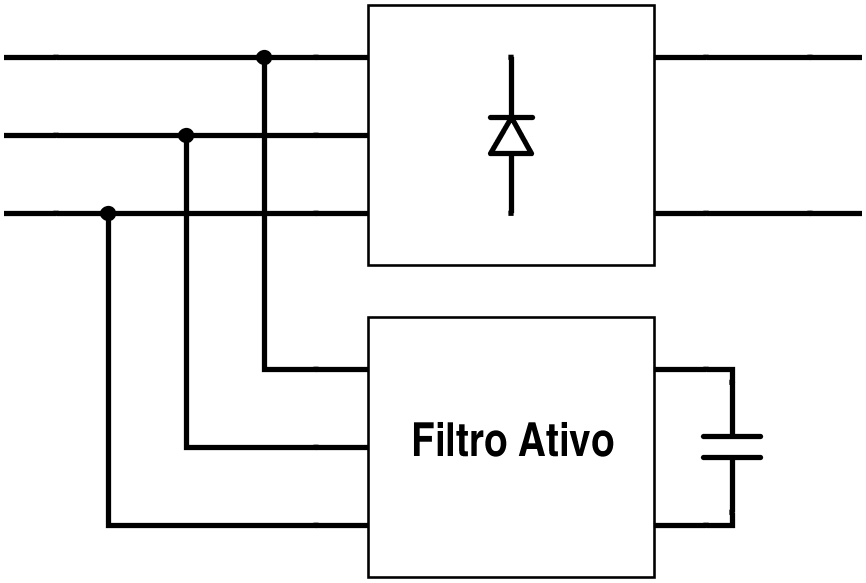
\includegraphics[width=0.65\textwidth]{Cap2/Figuras/shc_filtro_ativo.png}
	\caption{Filtro Ativo}
	\label{fig:sch_filtro_ativo}
\end{figure}

>>>>>>> origin/master
